\chapter{Software Infrastructure}
\epigraph{Look at you, hacker. A pathetic creature of meat and bone. Panting and
sweating as you run through my corridors. How can you challenge a perfect
immortal machine?}
{SHODAN - System Shock}
Creating a cyborg is a massive undertaking, thus a quite extensive software
suite has been created to make research feasible.
This chapter will focus on the more mundane engineering aspects of the software
developed for this thesis while the next chapter will focus on the
reconfigurable reservoir computing module at the heart of the project.
The following section contains an overview of the design philosophy, and an
overview of the individual components which are discussed in the remainder of
the chapter.
\section{Design Philosophy}
%
The physical cyborg is a loosely coupled system.
By communicating over network the neurons are not tied to a specific robot,
whatever lies beyond the network socket does not impact the lab setup.
%
Mirroring the physical setup, the software has a strong focus on loose coupling,
allowing different parts to be swapped out as long as interfaces between
components are adhered to.
%
A consequence of this design is, as described in the previous chapter, that the
``robot'' part of the cyborg can be swapped out, allowing different simulated
environments in addition to supporting physical robots.
A less obvious consequence is that the neural networks can be swapped out with
any other reservoir.
While the chief purpose of the software system is to interface with neurons,
being able to use a different reservoir is helpful both for testing and tuning
the software system, and for quantitatively investigating the differences between
neural cultures and other model reservoirs.
%
In short, the software architecture puts high emphasis on generic modular
components, and some parts are closer to a generic reservoir computing
framework, but most emphasis will be put on the neuron specific parts.
\subsection{Architecture}
An overview of the system architecture is shown in \ref{figOverview}.
\begin{figure}[h!]
  \centering
  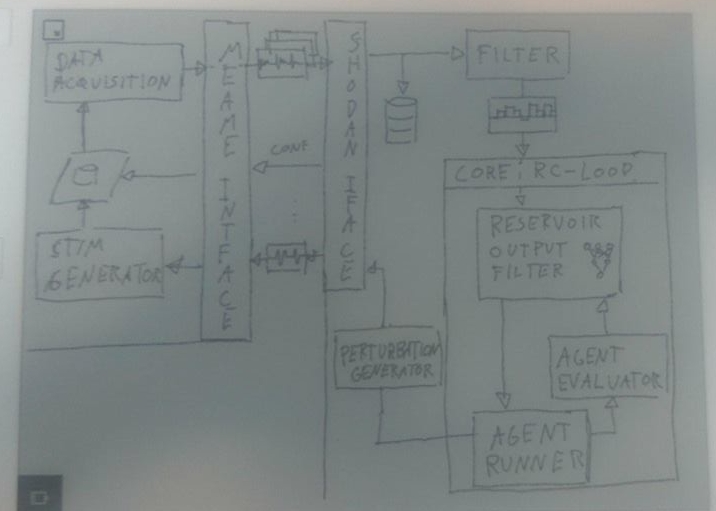
\includegraphics[width=0.5\textwidth]{fig/rm/sw_arc.jpg}
  \caption{Rough sketch.
    Should indicate the use of TCP/IP.
    Should show user interface.
    Final version will be done in inkscape.
  }
  \label{figOverview}
\end{figure}
The figure shows the closed dataloop, from neural measurements to perturbations.
First the data acquisition module collects voltage measurements from the neural
tissue, making it available over TCP/IP to any connected machine.
%
Next, the clients filtering module filters the raw waveform data, isolating
neural activity transformating high resolution waveform data into a simple
boolean spike or no spike format.
%
This spike data is then fed into the reservoir computer which outputs data to
the robot control module.
The format of this data is not specified, but for the robots used in this
project it is simply a single value specifying the desired turn rate.
%
Finally, the robot control module outputs sensory data, which is translated into
perturbations, i.e induced voltage spikes in the MEA.
These requests are transmitted over TCP/IP back to the reservoir.
%
Other than the core dataflow loop, the software system also presents a frontend
for the user to set up experiments and visualize the waveforms and a database
for storing and playing recorded data.
\subsection{Implementation}
The system today is comprised of two separate projects, \emph{MEAME} and
\emph{SHODAN} as seen in \ref{figOverview}.
Both projects have been implemented by the author specifically for the cyborg
project, and are available on github.
%
%
\section{MEAME}
The MEAME project is responsible for handling the tasks closest to the neural
reservoir, and is therefore installed on a computer directly connected to the
MEA2100 system.
MEAME is split into two subsystems, both exposed by a unified \emph{REST
  interface}, enabling access to the lab equipment via a protocol built on top
of HTTP.
The data acquisition part of MEAME is responsible for configuring recording
parameters such as samplerate and starting or stopping recordings.
It is built on top of a very thin windows only API provided by the equipment vendor, making
it abundantly clear that the cyborg project is pushing the equipment far beyond
its intended use, which at the same time is a point of pride and pain.
Once the data acquisition equipment has been configured MEAME exposes the
recorded data as a single continous stream which can be accessed via TCP.
Figure \ref{figLayout} shows the format of this data stream with only 3
electrodes, which must be demultiplexed by the receiver in order to separate
data into the 60 individual channels.
In order to stimulate the neurons, the HTTP interface can also handle stimuli
requests, which are executed on a realtime capable digital signal processor
which is embedded on the lab equipment itself.
\begin{figure}[h!]
  \centering
  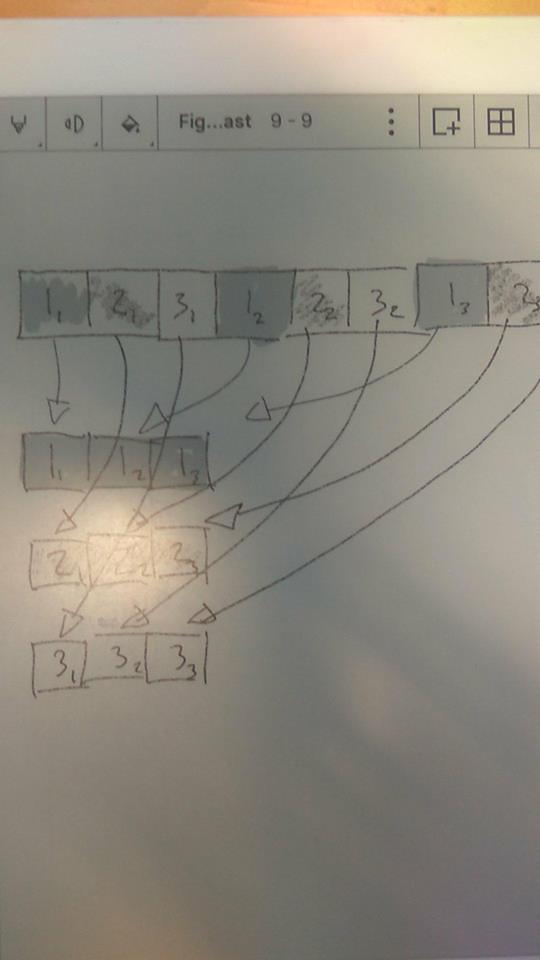
\includegraphics[width=0.5\textwidth]{fig/rm/waveform_segmentation.jpg}
  \caption{Rough sketch.
    Shows how data is transmitted.
  }
  \label{figLayout}
\end{figure}
\subsection{MEAME-DSP}
When MEAME receives a stimuli request this is communicated to the DSP through a
simple protocol implemented by directly writing to registers.
The DSP maintains a list of \emph{stim groups} which contain a list of electrode
numbers and a desired frequency.
Additionally the DSP is responsible for uploading which \emph{stimulus pattern}
to use when stimulating an electrode, however the DSP itself does not expose an
API for this purpose since uploading a stimulus pattern simply consists of
writing repeatedly to a single register, meaning this task is better handled at
a higher level.
A visual representation is given in \ref{figWaves} showing two stimulus groups.
\begin{figure}[h!]
  \centering
  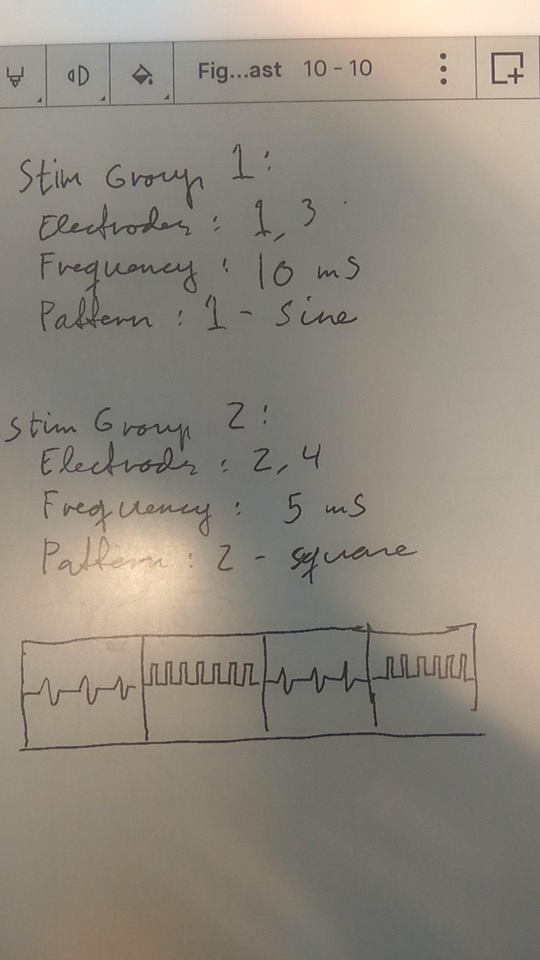
\includegraphics[width=0.5\textwidth]{fig/rm/dsp_config.jpg}
  \caption{Rough sketch.
    Some wavez
  }
  \label{figWaves}
\end{figure}
\section{SHODAN}
As shown in \ref{figOverview}, SHODAN is responsible for storage, filtering,
generating perturbations and maintaining the core RC loop.
To manage experiments SHODAN exposes a user interface that can be accessed in a
web-browser, allowing configuration of experiment parameters via the MEAME API,
real-time visualization of data and initiating experiments.
After an experiment has started SHODAN configures MEAME and starts streaming
data from MEAME.
This data is then consumed by the filtering module, which transforms the
high resolution voltage waveform data acquired from MEAME into a boolean format
discerning wether an electrode is spiking or not.
At the heart of SHODAN is the core RC loop which will be detailed next chapter.
% I don't know what to say here.
\cleardoublepage

%%% Local Variables:
%%% mode: latex
%%% TeX-master: "../main"
%%% End: